\section{Descrizione generale}

\begin{center}
	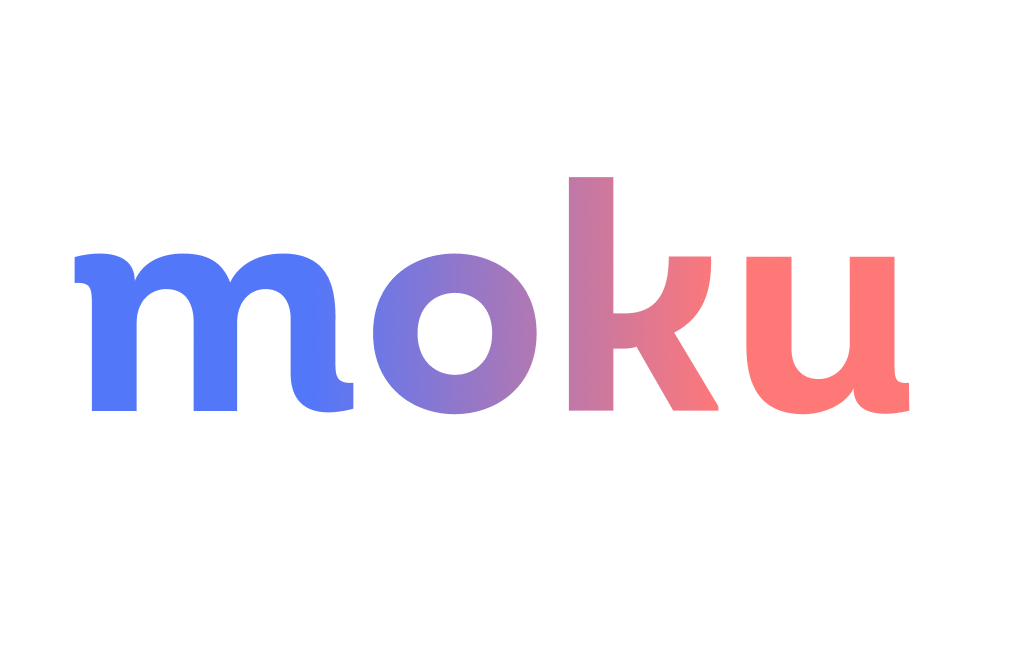
\includegraphics[height = 4cm]{moku-logo}
\end{center}
Moku S.r.l.\ è una start-up nata nel 2013 all'interno di un progetto supportato da H-Farm. Dopo aver abbandonato il progetto si è dedicata allo sviluppo software su commissione e consulenza, per poi allontanarsi definitivamente da H-Farm a settembre 2021, muovendo la sua sede dalla \emph{farm} a Roncade a quella attuale di Treviso. \\
L'azienda è in continua espansione e conta circa 20 dipendenti, la maggior parte con età inferiore ai 30 anni. Questo contribuisce a mantenere l'ambiente di lavoro stimolante e accogliente per tutti, permettendo di includere i diversi studenti che ogni anno svolgono il loro stage presso l'azienda. Per questi vengono attivate proposte di progetto per i ruoli di sviluppatore backend, sviluppatore frontend e sviluppatore mobile, all'interno di team interni che lavorano a progetti reali commissionati all'azienda.

\section{Modello di sviluppo}
\intro{Modello agile, Scrum, organizzazione dei team.}
